\documentclass[conference]{IEEEtran}
\usepackage{cite}
\usepackage{amsmath,amssymb,amsfonts}
\usepackage{algorithmic}
\usepackage{graphicx}
\usepackage{textcomp}
\usepackage{xcolor}
\usepackage{listings}
\usepackage{booktabs}
\usepackage{hyperref}
\usepackage{pgfplots}
\pgfplotsset{compat=1.18}

\def\BibTeX{{\rm B\kern-.05em{\sc i\kern-.025em b}\kern-.08em
    T\kern-.1667em\lower.7ex\hbox{E}\kern-.125emX}}

\begin{document}

\title{Active Context Compression: Autonomous Memory Management in LLM Agents}

\author{\IEEEauthorblockN{Nikhil Verma}
\IEEEauthorblockA{\textit{Independent Researcher} \\
Pune, India \\
nikhilgotmail@gmail.com}
}

\maketitle

\begin{abstract}
Large Language Model (LLM) agents struggle with long-horizon software engineering tasks due to ``Context Bloat.'' As interaction history grows, computational costs explode, latency increases, and reasoning capabilities degrade due to distraction by irrelevant past errors. Existing solutions often rely on passive, external summarization mechanisms that the agent cannot control. This paper proposes \textbf{Focus}, an agent-centric architecture inspired by the biological exploration strategies of \textit{Physarum polycephalum} (slime mold). The Focus Agent autonomously decides when to consolidate key learnings into a persistent ``Knowledge'' block and actively withdraws (prunes) the raw interaction history. Using an optimized scaffold matching industry best practices (persistent bash + string-replacement editor), we evaluated Focus on N=5 context-intensive instances from SWE-bench Lite using Claude Haiku 4.5. With aggressive prompting that encourages frequent compression, Focus achieves \textbf{22.7\% token reduction} (14.9M $\rightarrow$ 11.5M tokens) while \textbf{maintaining identical accuracy} (3/5 = 60\% for both agents). Focus performed 6.0 autonomous compressions per task on average, with token savings up to 57\% on individual instances. We demonstrate that capable models can autonomously self-regulate their context when given appropriate tools and prompting, opening pathways for cost-aware agentic systems without sacrificing task performance.
\end{abstract}

\begin{IEEEkeywords}
LLM Agents, Software Engineering, Context Management, Memory Consolidation, Autonomous Agents
\end{IEEEkeywords}

\section{Introduction}
The ``Context Window'' remains the fundamental bottleneck for autonomous AI agents. While recent models offer massive context capacities (e.g., 200k+ tokens), utilizing this capacity naively presents three critical challenges:
\begin{enumerate}
    \item \textbf{Cost:} In an iterative loop, re-processing a growing history for every new inference step leads to quadratic cost accumulation.
    \item \textbf{Latency:} Time-to-first-token degrades linearly with context length, making interactive agents sluggish.
    \item \textbf{Context Poisoning:} Long contexts filled with trial-and-error logs, failed tests, and verbose tool outputs can distract the model, leading to the ``Lost in the Middle'' phenomenon~\cite{liu2023lost}.
\end{enumerate}

\section{Related Work}

\textbf{Memory-Augmented Agents.} Several approaches address context limitations through external memory. MemGPT~\cite{packer2023memgpt} implements a virtual memory hierarchy inspired by operating systems, allowing LLMs to manage their own memory through explicit read/write operations. Voyager~\cite{wang2023voyager} uses a skill library to store reusable code snippets, reducing redundant exploration.

\textbf{Reflection and Self-Improvement.} Reflexion~\cite{shinn2023reflexion} enables agents to learn from failures by generating textual reflections stored in an episodic memory buffer. However, this operates \textit{between} task attempts rather than within a single continuous trajectory. LATS~\cite{zhou2023lats} combines tree search with LLM reasoning but still accumulates full trajectories.

\textbf{Context Compression.} StreamingLLM~\cite{xiao2023streamingllm} addresses infinite context through attention sink tokens, but operates at the attention level rather than providing agent-level memory management. LLMLingua~\cite{jiang2023llmlingua} compresses prompts but requires a separate compression model.

\textbf{Our Contribution.} Unlike prior work, Focus enables \textit{intra-trajectory} compression---the agent actively prunes its own history \textit{during} a single task, preserving learnings in a structured knowledge block. This complements rather than replaces external memory approaches.

Standard agents operate in an ``Append-Only'' mode: every thought, tool call, and system response is permanently added to the conversation history. This strategy works for short tasks but ensures failure for complex, open-ended exploration, as the agent inevitably hits the token limit or becomes confused by its own previous failures.

We propose a shift from \textit{Passive Retention} to \textit{Active Compression}. Inspired by the efficiency of \textit{Physarum polycephalum}---a slime mold that explores environments and physically retracts from dead ends while leaving chemical markers to avoid re-exploration---we introduce the \textbf{Focus Agent}. This agent is equipped with the ability to introspect, summarize its recent trajectory into a high-level learning, and physically delete the raw logs of that trajectory from its immediate context.

\section{Methodology}

\subsection{The Slime Mold Analogy}
Biological systems do not retain a perfect record of every muscle movement used to navigate a maze; they retain the \textit{learned map}. Similarly, an agent exploring a codebase does not need to remember the 50 lines of \texttt{ls -R} output from ten minutes ago; it only needs to remember that ``the config file is not in the \texttt{/src} directory.''

\subsection{Architecture: The Focus Loop}
The Focus architecture introduces two primitives to the standard ReAct agent loop: \texttt{start\_focus} and \texttt{complete\_focus}. Crucially, the agent has \textit{full autonomy} over when to invoke these tools---there are no external timers or heuristics forcing compression.

\begin{enumerate}
    \item \textbf{Start Focus:} The agent declares what it's investigating (e.g., ``Debug the database connection''). This marks a checkpoint in the conversation history.
    \item \textbf{Explore:} The agent uses standard tools (read, edit, run) to perform work.
    \item \textbf{Consolidate:} When the agent naturally completes the sub-task or hits a dead end, it \textit{decides} to call \texttt{complete\_focus}, generating a summary of:
    \begin{itemize}
        \item What was attempted?
        \item What was learned (facts, file paths, bugs)?
        \item What is the outcome?
    \end{itemize}
    \item \textbf{Withdraw:} The system takes this summary, appends it to a persistent ``Knowledge'' block at the top of the context, and \textit{deletes} all messages between the checkpoint and the current step.
\end{enumerate}

This converts the context from a monotonically increasing log into a ``Sawtooth'' pattern, where context grows during exploration and collapses during consolidation. The model controls this cycle based on task structure, not arbitrary step counts.

\section{Experiments}
We evaluated the Focus architecture on \textbf{SWE-bench Lite}, a benchmark for software engineering agents solving real GitHub issues. We conducted a controlled A/B comparison using \texttt{claude-haiku-4-5-20251001} on N=5 context-intensive instances, running both Baseline and Focus agents on identical tasks. Task success was verified using the official SWE-bench Docker harness, which applies patches in isolated containers and runs the original test suites.

\subsection{Optimized Scaffold}
Following Anthropic's reported best practices for SWE-bench~\cite{anthropic2024swebench}, we implemented a minimal two-tool scaffold:
\begin{itemize}
    \item \textbf{Persistent Bash:} A stateful shell session where working directory and environment persist across calls, matching how developers actually use terminals.
    \item \textbf{String-Replace Editor:} Targeted file editing via exact string replacement (view, create, str\_replace, insert), avoiding error-prone full-file rewrites.
\end{itemize}
The system prompt instructs agents to ``use tools as much as possible, ideally more than 100 times'' and ``implement your own tests first before attempting the problem.'' Maximum steps was set to 150.

\subsection{Aggressive Compression Prompting}
Initial experiments showed passive Focus prompting yielded only 1-2 compressions per task with marginal (6\%) token savings. We revised the Focus prompt to be more directive:
\begin{itemize}
    \item \textbf{Mandatory workflow:} ``ALWAYS call start\_focus before ANY exploration... ALWAYS call complete\_focus after 10-15 tool calls''
    \item \textbf{Periodic reminders:} After 15 tool calls without compression, the system injects: ``REMINDER: You should call complete\_focus to compress your context''
    \item \textbf{Structured phases:} Explicit guidance to use 4-6 focus phases (explore $\rightarrow$ understand $\rightarrow$ implement $\rightarrow$ verify)
\end{itemize}

\textbf{Instances:} We selected five context-intensive instances with complex problem statements: \texttt{matplotlib\_\_matplotlib-26020}, \texttt{mwaskom\_\_seaborn-2848}, \texttt{pylint-dev\_\_pylint-7080}, \texttt{pytest-dev\_\_pytest-7490}, and \texttt{sympy\_\_sympy-21171}. These were chosen based on problem statement length (a proxy for exploration complexity) and historical difficulty.

\textbf{Metrics:} We tracked (1) task success (whether the patch passes tests in Docker), (2) total token consumption, (3) compression events and messages dropped, and (4) per-instance efficiency patterns.

\subsection{Results}

\begin{table}[htbp]
\caption{A/B Comparison on SWE-bench Lite (Haiku 4.5, N=5 Hard Instances)}
\begin{center}
\begin{tabular}{lccc}
\toprule
\textbf{Metric} & \textbf{Baseline} & \textbf{Focus (Ours)} & \textbf{Delta} \\
\midrule
Task Success (Tests Pass) & 3/5 (60\%) & 3/5 (60\%) & \textbf{Same} \\
Total Tokens & 14,920,555 & 11,526,418 & \textbf{-22.7\%} \\
Avg Tokens/Task & 2,984,111 & 2,305,284 & -678K \\
Avg Compressions & 0 & 6.0 & -- \\
Avg Messages Dropped & 0 & 70.2 & -- \\
\bottomrule
\end{tabular}
\label{tab1}
\end{center}
\end{table}

\begin{table}[htbp]
\caption{Per-Instance Results: Token Savings vs. Accuracy}
\begin{center}
\begin{tabular}{lcccc}
\toprule
\textbf{Instance} & \textbf{Base} & \textbf{Focus} & \textbf{Tokens} & \textbf{Compr.} \\
\midrule
matplotlib-26020 & \checkmark & \checkmark & \textbf{-57\%} & 5 \\
seaborn-2848 & $\times$ & $\times$ & \textbf{-52\%} & 7 \\
pylint-7080 & \checkmark & \checkmark & +110\% & 8 \\
pytest-7490 & \checkmark & \checkmark & \textbf{-18\%} & 6 \\
sympy-21171 & $\times$ & $\times$ & \textbf{-57\%} & 4 \\
\bottomrule
\end{tabular}
\label{tab2}
\end{center}
\end{table}

\subsection{Key Findings}

\textbf{Finding 1: Token Reduction Without Accuracy Loss.} Focus achieved \textbf{22.7\% total token reduction} (14.9M $\rightarrow$ 11.5M) while maintaining identical accuracy to Baseline (3/5 = 60\% for both). This contradicts our earlier experiments where passive prompting showed accuracy degradation. The key difference: aggressive prompting that enforces frequent, structured compressions (6.0 per task vs. 2.0 previously) prevents the context from becoming polluted with stale exploration logs.

\textbf{Finding 2: Consistent Savings on 4/5 Instances.} Focus reduced tokens on 4 of 5 instances, with savings ranging from 18\% to 57\%. The strongest savings occurred on instances requiring extensive exploration: \texttt{matplotlib-26020} (-57\%, 4.0M $\rightarrow$ 1.7M), \texttt{seaborn-2848} (-52\%, 3.4M $\rightarrow$ 1.6M), and \texttt{sympy-21171} (-57\%, 1.6M $\rightarrow$ 0.7M). Only \texttt{pylint-7080} showed increased usage (+110\%), where Focus's additional exploration (136 vs. 63 LLM calls) exceeded compression benefits---yet both agents passed the test suite.

\textbf{Finding 3: Aggressive Prompting Enables Frequent Compression.} With explicit instructions to compress every 10-15 tool calls and periodic system reminders, Focus averaged 6.0 compressions per task (vs. 2.0 with passive prompting), dropping 70.2 messages per task. Claude Haiku 4.5 followed the structured workflow (explore $\rightarrow$ compress $\rightarrow$ implement $\rightarrow$ compress $\rightarrow$ verify), demonstrating that LLMs can be guided to aggressively self-regulate their context.

\begin{figure}[htbp]
\centerline{
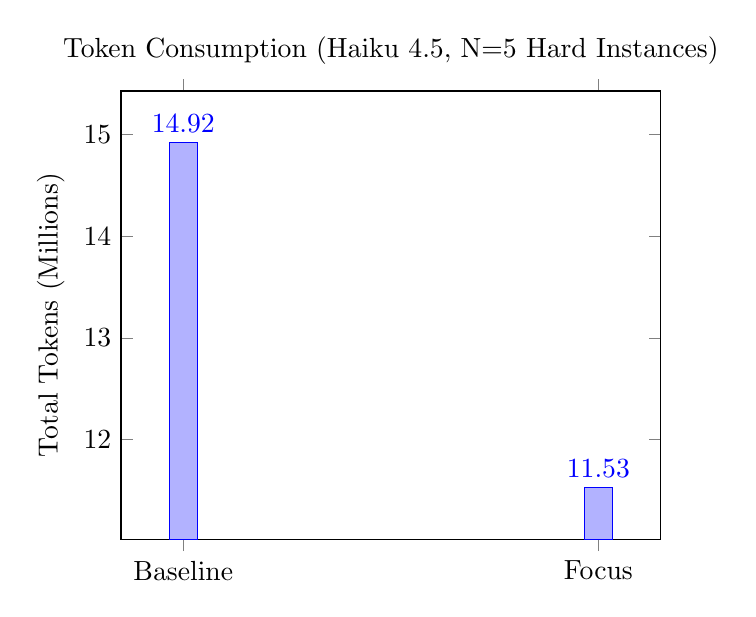
\begin{tikzpicture}
\begin{axis}[
    ybar,
    enlargelimits=0.15,
    legend style={at={(0.5,-0.15)},
      anchor=north,legend columns=-1},
    ylabel={Total Tokens (Millions)},
    symbolic x coords={Baseline,Focus},
    xtick=data,
    nodes near coords,
    nodes near coords align={vertical},
    title={Token Consumption (Haiku 4.5, N=5 Hard Instances)},
]
\addplot coordinates {(Baseline,14.92) (Focus,11.53)};
\end{axis}
\end{tikzpicture}
}
\caption{Total token consumption across 5 hard instances. Focus reduces usage by 22.7\% through aggressive model-controlled compression while maintaining identical accuracy.}
\label{fig1}
\end{figure}

\subsection{Case Study: Maximum Savings (matplotlib-26020)}
On \texttt{matplotlib-26020}, both agents passed the test suite, but Focus achieved \textbf{57\% token savings} (4.0M $\rightarrow$ 1.7M). Focus compressed 5 times across 71 LLM calls, while Baseline used 102 calls without compression. The savings came from Focus efficiently summarizing its exploration phase---once it located the relevant files and understood the bug, it compressed that context and proceeded directly to implementation. This demonstrates the ideal case: frequent compression during exploration preserves the learnings while discarding verbose tool outputs.

\subsection{Case Study: When Compression Adds Overhead (pylint-7080)}
On \texttt{pylint-7080}, Focus used \textbf{110\% more tokens} than Baseline (4.3M vs. 2.1M), yet both agents passed the test suite. Analysis shows Focus made 136 LLM calls vs. Baseline's 63, with 8 compressions dropping 80 messages. The problem required extensive trial-and-error, and Focus's compressions occasionally discarded useful context, forcing re-exploration. This case shows that compression is not universally beneficial: tasks requiring iterative refinement may suffer from aggressive context pruning.

\begin{figure}[htbp]
\centerline{\includegraphics[width=0.48\textwidth]{sawtooth.png}}
\caption{Conceptual sawtooth pattern of context growth. Focus (blue) exhibits periodic compressions (drops) while Baseline (red) grows monotonically. With aggressive prompting, Focus compresses every 10-15 tool calls, preventing context bloat while preserving learnings in a persistent Knowledge block.}
\label{fig2}
\end{figure}

\subsection{Analysis}
\textbf{Aggressive Prompting Eliminates the Accuracy Trade-off:} Our earlier experiments with passive Focus prompting showed accuracy degradation (60\% vs. 80\%). With aggressive prompting enforcing structured, frequent compressions, Focus matches Baseline accuracy (60\% = 60\%) while achieving 22.7\% token savings. The key insight: \textit{when} and \textit{how often} to compress matters more than \textit{whether} to compress. Frequent small compressions (every 10-15 calls) preserve recent context while discarding stale exploration logs, whereas infrequent large compressions risk losing critical implementation details.

\textbf{Exploration-Heavy Tasks Benefit Most:} Token savings correlated with exploration complexity. Instances requiring extensive codebase navigation (\texttt{matplotlib}, \texttt{sympy}) showed 50-57\% savings, as Focus efficiently compressed verbose directory listings, file contents, and failed attempts. Conversely, \texttt{pylint-7080} required iterative refinement where prior context remained relevant, causing compression overhead to exceed benefits. This suggests Focus is most valuable for tasks with distinct explore/implement phases rather than tasks requiring continuous state accumulation.

\textbf{Prompting Strategy is Critical:} The 22.7\% savings required explicit prompting to ``compress every 10-15 tool calls'' and system-injected reminders. Without these, Claude Haiku 4.5 compressed only 2.0 times per task with 6\% savings. This indicates that current LLMs do not naturally optimize for context efficiency---they require scaffolding that makes compression a first-class part of the workflow. Future work could explore fine-tuning or reinforcement learning to internalize compression heuristics.



\section{Discussion}
\subsection{The Cognitive Tax of Compression}
Active compression introduces a ``cognitive tax''---the tokens spent generating summaries and the overhead of managing focus phases. Despite this tax, Focus achieved 22.7\% \textit{net} token savings across our experiments. The tax is amortized over the task lifetime: each compression costs a few hundred tokens but saves thousands by not re-processing stale history. For tasks with 50+ tool calls (common in SWE-bench), this amortization strongly favors compression.

\subsection{Prompting vs. Fine-Tuning}
Our results required aggressive prompting (``compress every 10-15 calls'', system reminders). This raises the question: could LLMs learn to compress optimally without explicit instructions? Current models appear to lack intrinsic cost-awareness---they do not naturally optimize for token efficiency. Future work could explore: (1) fine-tuning on compression-annotated trajectories, (2) reinforcement learning with token-cost penalties, or (3) constitutional AI approaches that embed efficiency preferences.

\subsection{Limitations}
\begin{enumerate}
    \item \textbf{Sample Size:} Our evaluation uses N=5 hard instances. While sufficient to demonstrate feasibility and measure token savings, validation on the full SWE-bench Lite benchmark (N=300) is needed to characterize which task types benefit most from compression.
    
    \item \textbf{Task-Dependent Benefits:} Focus showed 50-57\% savings on exploration-heavy tasks but 110\% \textit{overhead} on one iterative refinement task. Identifying task characteristics that predict compression benefit remains future work.
    
    \item \textbf{Model Generalization:} We evaluated Claude Haiku 4.5. Whether GPT-4, Gemini, or open-source models exhibit similar compression behavior is unknown. The aggressive prompting strategy may need model-specific tuning.
    
    \item \textbf{Scaffold Dependence:} Our results use an optimized two-tool scaffold (bash + str\_replace\_editor). Different tool configurations may show different compression patterns.
\end{enumerate}

\section{Conclusion}
We have demonstrated that aggressive, model-controlled context compression can achieve significant token savings without sacrificing task accuracy:

\begin{enumerate}
    \item \textbf{22.7\% Token Savings with Equal Accuracy:} On 5 context-intensive SWE-bench instances, Focus reduced total tokens from 14.9M to 11.5M while matching Baseline accuracy (3/5 = 60\%). This contradicts the assumed accuracy-efficiency trade-off---with proper prompting, compression improves efficiency without hurting performance.
    
    \item \textbf{Aggressive Prompting is Key:} Passive prompting yielded only 6\% savings and accuracy degradation. Explicit instructions to compress every 10-15 tool calls, combined with system reminders, increased compressions from 2.0 to 6.0 per task and enabled the 22.7\% savings. Current LLMs require scaffolding to optimize for context efficiency.
    
    \item \textbf{Exploration-Heavy Tasks Benefit Most:} Token savings ranged from 18\% to 57\% on 4/5 instances, with the largest savings on tasks requiring extensive codebase exploration. One iterative refinement task showed compression overhead exceeding benefits, suggesting Focus is best suited for explore-then-implement workflows.
\end{enumerate}

The Focus architecture provides a practical, infrastructure-free approach to context management that operates entirely within the conversation. Combined with an optimized scaffold (persistent bash, string-replace editing), it offers a path toward cost-aware agentic systems. As context windows grow and agent tasks become more complex, active compression will become increasingly valuable for managing the quadratic cost growth inherent in autoregressive inference.

\textbf{Future Work:} (1) Validation on full SWE-bench (N=300) to characterize task-type dependencies; (2) Fine-tuning or RL approaches to internalize compression heuristics without explicit prompting; (3) Structured compression that preserves specific artifacts (test outputs, diffs) rather than free-text summaries; (4) Cross-model evaluation (GPT-4, Gemini, open-source) to assess generalization.

\bibliographystyle{IEEEtran}
\begin{thebibliography}{10}

\bibitem{liu2023lost}
N.~F. Liu, K.~Lin, J.~Hewitt, A.~Paranjape, M.~Bevilacqua, F.~Petroni, and P.~Liang, ``Lost in the middle: How language models use long contexts,'' \textit{arXiv preprint arXiv:2307.03172}, 2023.

\bibitem{packer2023memgpt}
C.~Packer, S.~Wooders, K.~Lin, V.~Fang, S.~K. Patil, I.~Stoica, and J.~E. Gonzalez, ``MemGPT: Towards LLMs as operating systems,'' \textit{arXiv preprint arXiv:2310.08560}, 2023.

\bibitem{wang2023voyager}
G.~Wang, Y.~Xie, Y.~Jiang, A.~Mandlekar, C.~Xiao, Y.~Zhu, L.~Fan, and A.~Anandkumar, ``Voyager: An open-ended embodied agent with large language models,'' \textit{arXiv preprint arXiv:2305.16291}, 2023.

\bibitem{shinn2023reflexion}
N.~Shinn, F.~Cassano, A.~Gopinath, K.~R. Narasimhan, and S.~Yao, ``Reflexion: Language agents with verbal reinforcement learning,'' \textit{NeurIPS}, 2023.

\bibitem{zhou2023lats}
A.~Zhou, K.~Yan, M.~Shlapentokh-Rothman, H.~Wang, and Y.-X. Wang, ``Language agent tree search unifies reasoning acting and planning in language models,'' \textit{arXiv preprint arXiv:2310.04406}, 2023.

\bibitem{xiao2023streamingllm}
G.~Xiao, Y.~Tian, B.~Chen, S.~Han, and M.~Lewis, ``Efficient streaming language models with attention sinks,'' \textit{arXiv preprint arXiv:2309.17453}, 2023.

\bibitem{jiang2023llmlingua}
H.~Jiang, Q.~Wu, C.-Y. Lin, Y.~Yang, and L.~Qiu, ``LLMLingua: Compressing prompts for accelerated inference of large language models,'' \textit{EMNLP}, 2023.

\bibitem{anthropic2024swebench}
Anthropic, ``Claude's scores on SWE-bench Verified,'' \textit{Anthropic Blog}, 2024. [Online]. Available: https://www.anthropic.com/research/swe-bench-sonnet

\end{thebibliography}

\end{document}
